%!TEX root = ../book_ML.tex

\def\R{\mathbb{R}}
\newpage
\section{Bảng các ký hiệu}
Các ký hiệu sử dụng trong sách được liệt kê trong Bảng~\ref{tab:notation}.

\begin{table}[h]
    \caption{Các quy ước ký hiệu và tên gọi được sử dụng trong báo cáo}
    \label{tab:notation}
    \centering
    \begin{tabular}{|c|l|}
    \hline 
    Ký hiệu & Ý nghĩa  \\ \hline 
    \hline 
    $x, y, N, k$ & in nghiêng, thường hoặc hoa, là các số vô hướng \\ \hline
    $\bx, \by$ & in đậm, chữ thường, là các vector  \\ \hline
    $\bX, \bY$ & in đậm, chữ hoa, là các ma trận  \\ \hline
    $\R$ & tập hợp các số thực \\ \hline 
    $\mathbb{N}$ & tập hợp các số tự nhiên \\ \hline 
    $\mathbb{C}$ & tập hợp các số phức \\ \hline 
    $\R^{m}$ & tập hợp các vector thực có $m$ phần tử \\ \hline 
    $\R^{m\times n}$ &tập hợp các ma trận thực có $m$ hàng, $n$ cột \\ \hline
    $\mathbb{S}^n$ & tập hợp các ma trận vuông đối xứng bậc $n$ \\ \hline 
    $\mathbb{S}^n_{+}$ & tập hợp các ma trận nửa xác định dương bậc $n$ \\
    \hline 
    $\mathbb{S}^n_{++}$ & tập hợp các ma trận xác định dương bậc $n$ \\ \hline 
    $ \in $ & phần tử thuộc tập hợp \\ \hline 
    $ \exists $ & tồn tại \\ \hline 
    $ \forall $ & mọi \\ \hline 
    $ \triangleq$ & ký hiệu là/bởi. Ví dụ $a\triangleq f(x)$ nghĩa là ``ký hiệu
    $f(x)$ bởi $a$''. \\ \hline 
    $x_i$ & phần tử thứ $i$ (tính từ 1) của vector $\bx$ \\ \hline 
    $\sgn(x)$ & hàm xác định dấu. Bằng 1 nếu $x \geq 0$, bằng -1 nếu $x < 0$. \\ \hline
    $\exp(x)$ & $e^x$ \\ \hline
    $\log(x)$ & logarit \textit{tự nhiên} của số thực dương $x$ \\ \hline
    $\displaystyle \argmin_xf(x)$ & giá trị của $x$ để hàm $f(x)$ đạt giá trị nhỏ nhất \\ \hline 
    $\displaystyle \argmax_xf(x)$ & giá trị của $x$ để hàm $f(x)$ đạt giá trị lớn nhất \\ \hline 
    % $a_{ij}$ & phần tử hàng thứ $i$, cột thứ $j$ của ma trận $\bA$ \\ \hline 
    % $\bA^T$ & chuyển vị của ma trận $\bA$ \\ \hline 
    % $\bA^H$ & chuyển vị liên hợp (Hermitian) của ma trận phức $\bA$ \\ \hline 
    % $\bA^{-1}$ & nghịch đảo của ma trận vuông $\bA$, nếu tồn tại \\ \hline 
    % $\bA^{\dagger}$ & giả nghịch đảo của ma trận không nhất thiết vuông $\bA$ \\
    % \hline 
    % $\bA^{-T}$ & chuyển vị của nghịch đảo của ma trận $\bA$, nếu tồn tại \\ \hline 
    % $\|\bx\|_p$ & $\ell_p$ norm của vector $\bx$ \\ \hline  
    % $\|\bA\|_F$ &  Frobenius norm của ma trận $\bA$ \\ \hline 
    % $ \diag(\bA)$ & đường chéo chính của ma trận $\bA$ \\ \hline 
    % $\trace(\bA)$ & trace của ma trận $\bA$ \\ \hline 
    % $\det(\bA)$ & định thức của ma trận vuông $\bA$ \\ \hline 
    % $\text{rank}(\bA)$ & hạng của ma trận $\bA$ \\ \hline 
    o.w & \textit{otherwise}  --  trong các trường hợp còn lại \\ \hline 
    $\displaystyle\frac{\partial f}{\partial x}$ & đạo hàm của hàm số $f$ theo $x \in \R$ \\ \hline
    $\nabla_{\bx}f$ & gradient của hàm số $f$ theo $\bx$ ($\bx$ là vector hoặc ma trận) \\ \hline 
    $\nabla^2_{\bx}f$ & gradient bậc hai của hàm số $f$ theo $\bx$, còn được gọi là \textit{Hesse} \\ \hline 
    $\odot$ & \makecell{Hadamard product (elemenwise product). Phép nhân từng phần tử \\ của hai vector hoặc ma trận cùng kích thước.} \\ \hline 
    $\propto$ & tỉ lệ với \\ \hline 
    % v.v. & vân vân \\ \hline 
    %%%%%%%
    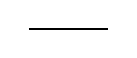
\begin{tikzpicture}
    \draw [thick] (0, 0) -- (1, 0); 
    \end{tikzpicture}
    & đường nét liền \\ \hline 

    %%%%%%%
    \begin{tikzpicture}
    \draw [very thick, dashed] (0, 0) -- (1, 0); 
    \end{tikzpicture}
    & đường nét đứt \\ \hline 

    %%%%%%%
    \begin{tikzpicture}
    \draw [very thick, dotted] (0, 0) -- (1, 0); 
    \end{tikzpicture}
    & đường nét chấm (đường chấm chấm)\\ \hline 

    %%%%%%%
    \begin{tikzpicture}
    \draw [very thick, dash pattern={on 7pt off 2pt on 1pt off 3pt}] (0,0) -- (1,0);
    \end{tikzpicture}
    & đường chấm gạch\\ \hline 
    %%%%%%%
    % \\[-3mm]
    % \vspace{1em}
    \begin{tikzpicture}[yshift = -1cm]
    \draw [pattern = dots] (0,0) rectangle (1,.4);
    \end{tikzpicture}
    & nền chấm\\\hline 
    %%%%%%%
    % \\[-1em]
    % \vspace{1em}
    \begin{tikzpicture}
    \draw [pattern = custom north west lines] (0,0) rectangle (1,.4);
    \end{tikzpicture}
    & nền sọc chéo\\ \hline 



    \end{tabular}
 \end{table} 